\documentclass[aspectratio=169,10pt]{beamer}
\usetheme{Madrid}
\usecolortheme{default}
\usepackage[T1]{fontenc}
\usepackage[utf8]{inputenc}
\usepackage{lmodern}
\usepackage{booktabs}
\usepackage{graphicx}

\title{Consumer Complaint Classification under Small-Data Constraints}
\subtitle{Mini-Project Presentation}
\author{Khayrislamov Timur \and Petrenko Maksim}
\institute{Natural Language Processing (NLP) in Python}
\date{}

\begin{document}

\begin{frame}
  \titlepage
\end{frame}

\begin{frame}{Research Question and Task}
\begin{itemize}
    \item \textbf{Goal:} predict the \textit{product category} from each consumer complaint narrative.
    \item \textbf{Setting:} balanced 5-class classification problem under \textbf{small-data constraints}.
    \item \textbf{Questions:}
    \begin{itemize}
        \item How does performance change as the number of labeled examples per class increases?
        \item Are pretrained embeddings better than locally trained embeddings in the low-data regime?
    \end{itemize}
    \item \textbf{Classes:} Bank account or service, Credit card, Credit reporting, Debt collection, Mortgage.
\end{itemize}
\end{frame}

\begin{frame}{Models and Experimental Setup}
\begin{columns}[T,totalwidth=\textwidth]
\column{0.50\textwidth}
\textbf{Models}
\begin{itemize}
    \item TF--IDF + Logistic Regression
    \item Local Word2Vec + MLP
    \item Pretrained GloVe + MLP
\end{itemize}

\column{0.50\textwidth}
\textbf{Evaluation}
\begin{itemize}
    \item Main metric: Macro F1
    \item Accuracy also reported
    \item Balanced subset sizes: 100, 300, 600, 1000, 2000 per class
    \item 3 random seeds per size
    \item Stratified train/validation/test split
\end{itemize}
\end{columns}

\vspace{0.35cm}
\textbf{Motivation:} compare a strong classical sparse baseline against embedding-based document representations.
\end{frame}

\begin{frame}{Single Full-Data Run}
\centering
\begin{tabular}{lcc}
\toprule
Model & Accuracy & Macro F1 \\
\midrule
TF--IDF + Logistic Regression & 0.8679 & 0.8680 \\
Local Word2Vec + MLP & 0.8435 & 0.8423 \\
Pretrained GloVe + MLP & 0.7454 & 0.7427 \\
\bottomrule
\end{tabular}

\vspace{0.4cm}
\begin{itemize}
    \item TF--IDF is the strongest overall model.
    \item Local Word2Vec is competitive, but still below the sparse baseline.
    \item Pretrained GloVe is clearly the weakest approach.
\end{itemize}
\end{frame}

\begin{frame}{Main Result: Macro F1 Across Dataset Sizes}
\centering
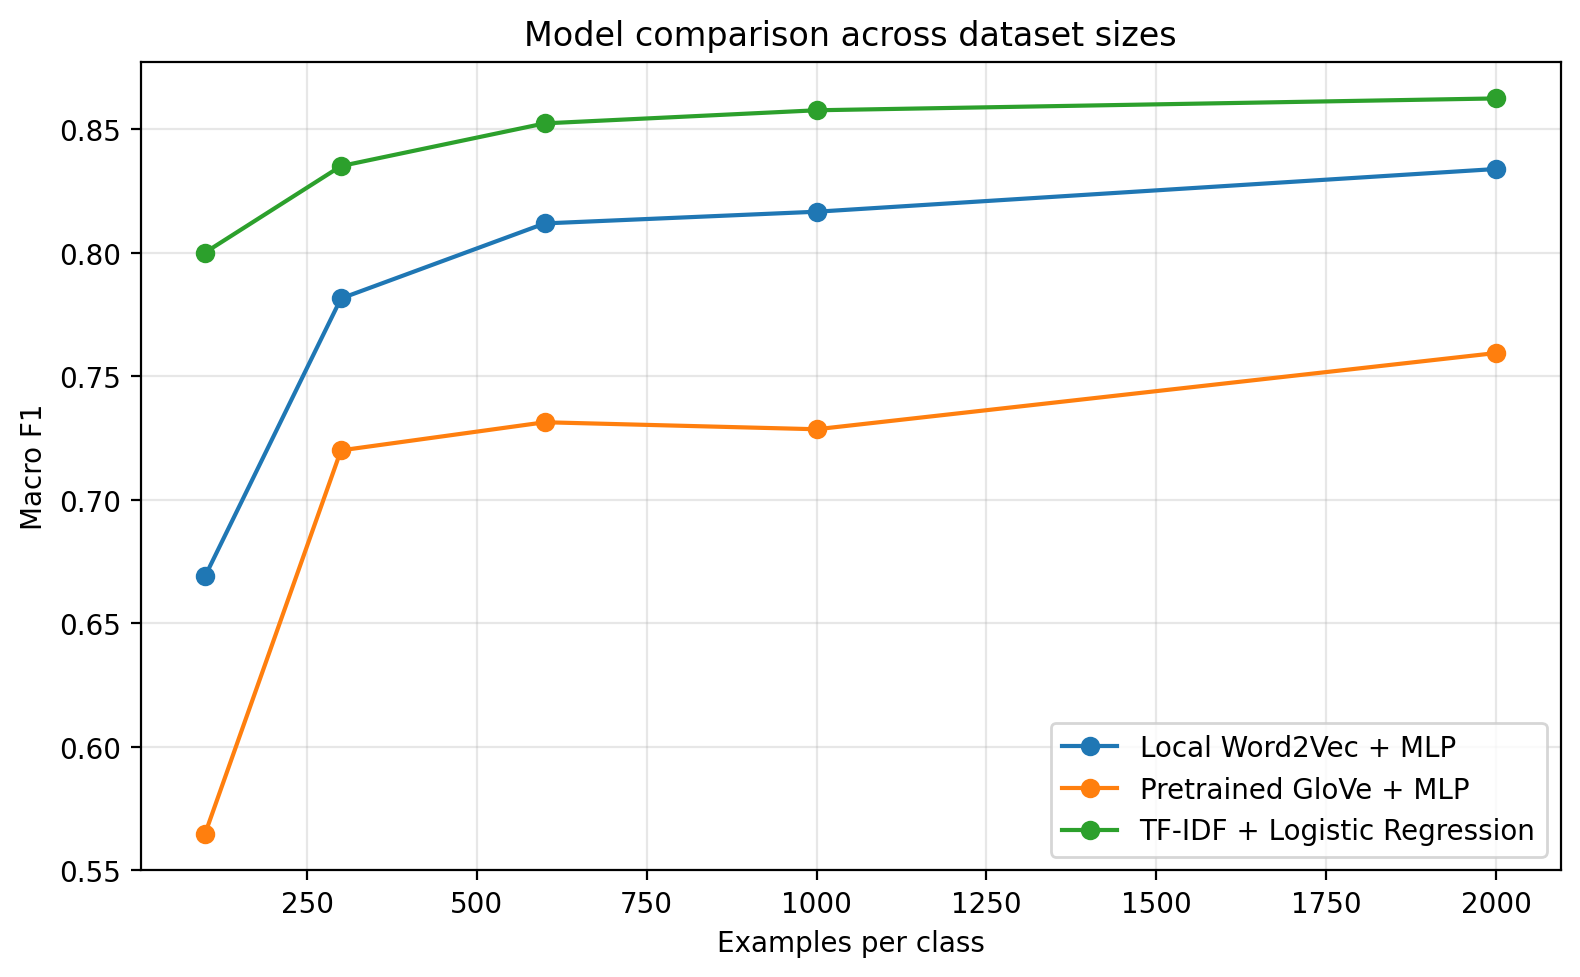
\includegraphics[width=0.92\linewidth]{../artifacts/model_comparison_compact.png}

\vspace{0.2cm}
\small TF--IDF stays on top at every data size; Local Word2Vec improves steadily; Pretrained GloVe remains weakest.
\end{frame}

\begin{frame}{Repeated Study Curves with Variability}
\centering
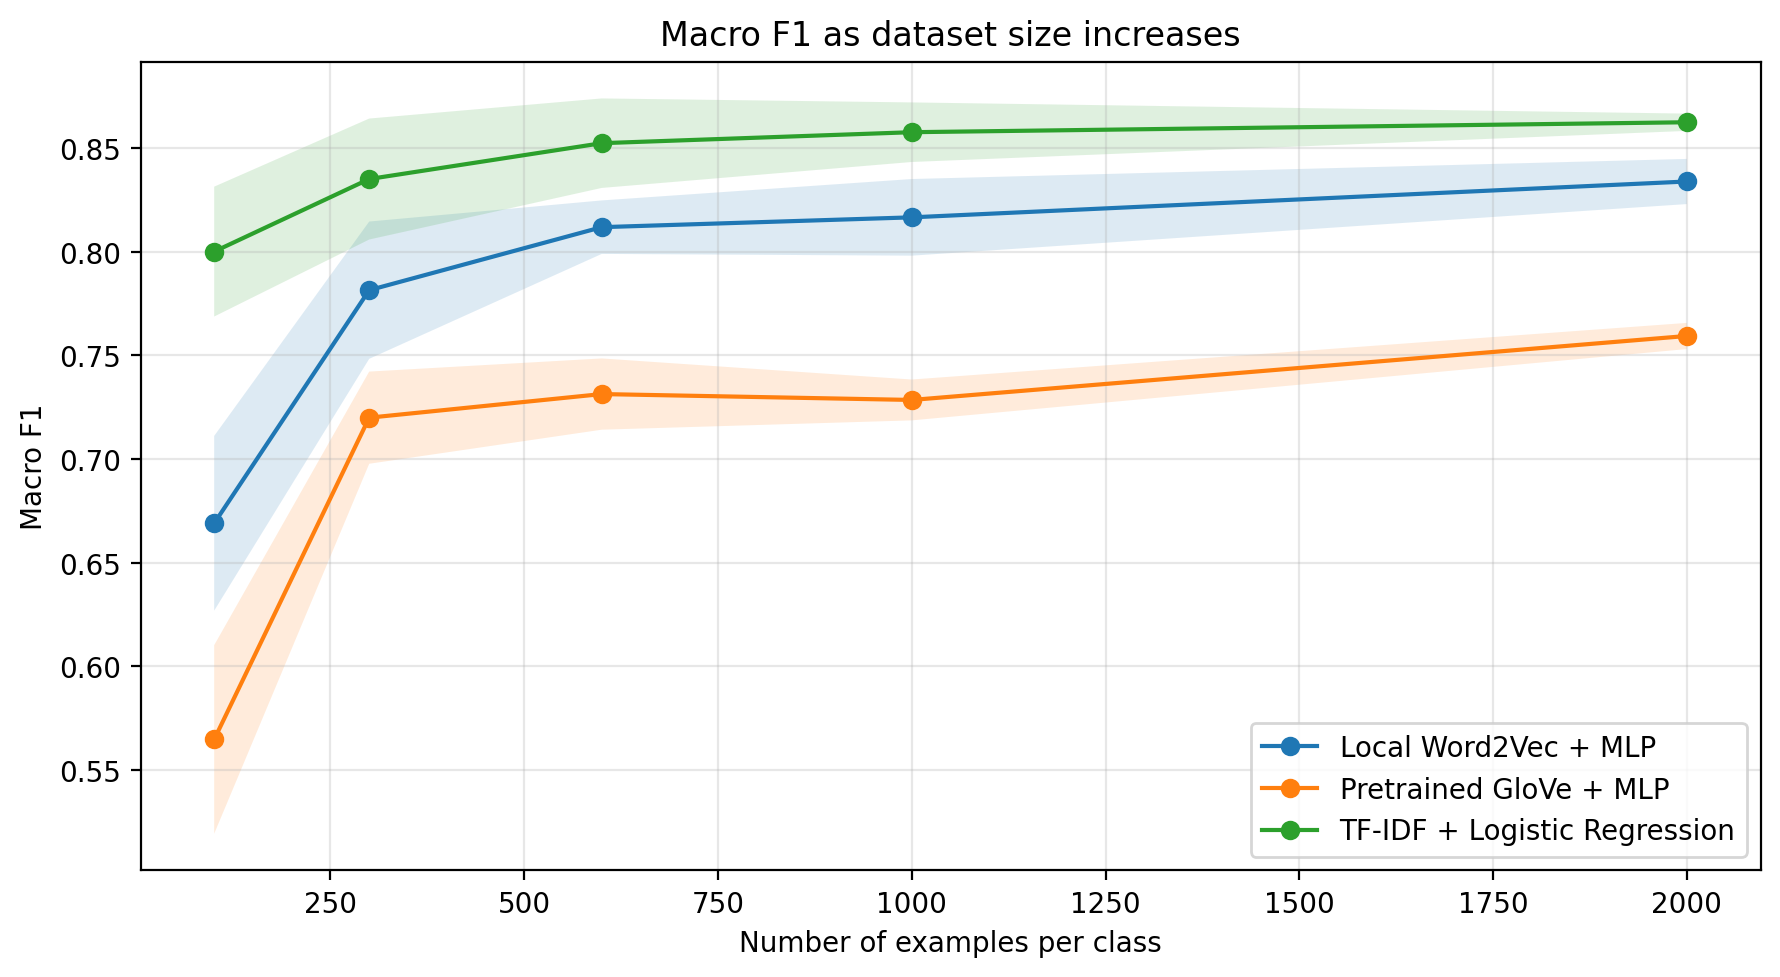
\includegraphics[width=0.92\linewidth]{../artifacts/macro_f1_vs_size.png}

\vspace{0.15cm}
\small Mean $\pm$ standard deviation across three random seeds. Variance shrinks as dataset size increases.
\end{frame}

\begin{frame}{Error Analysis of the Best Model}
\centering
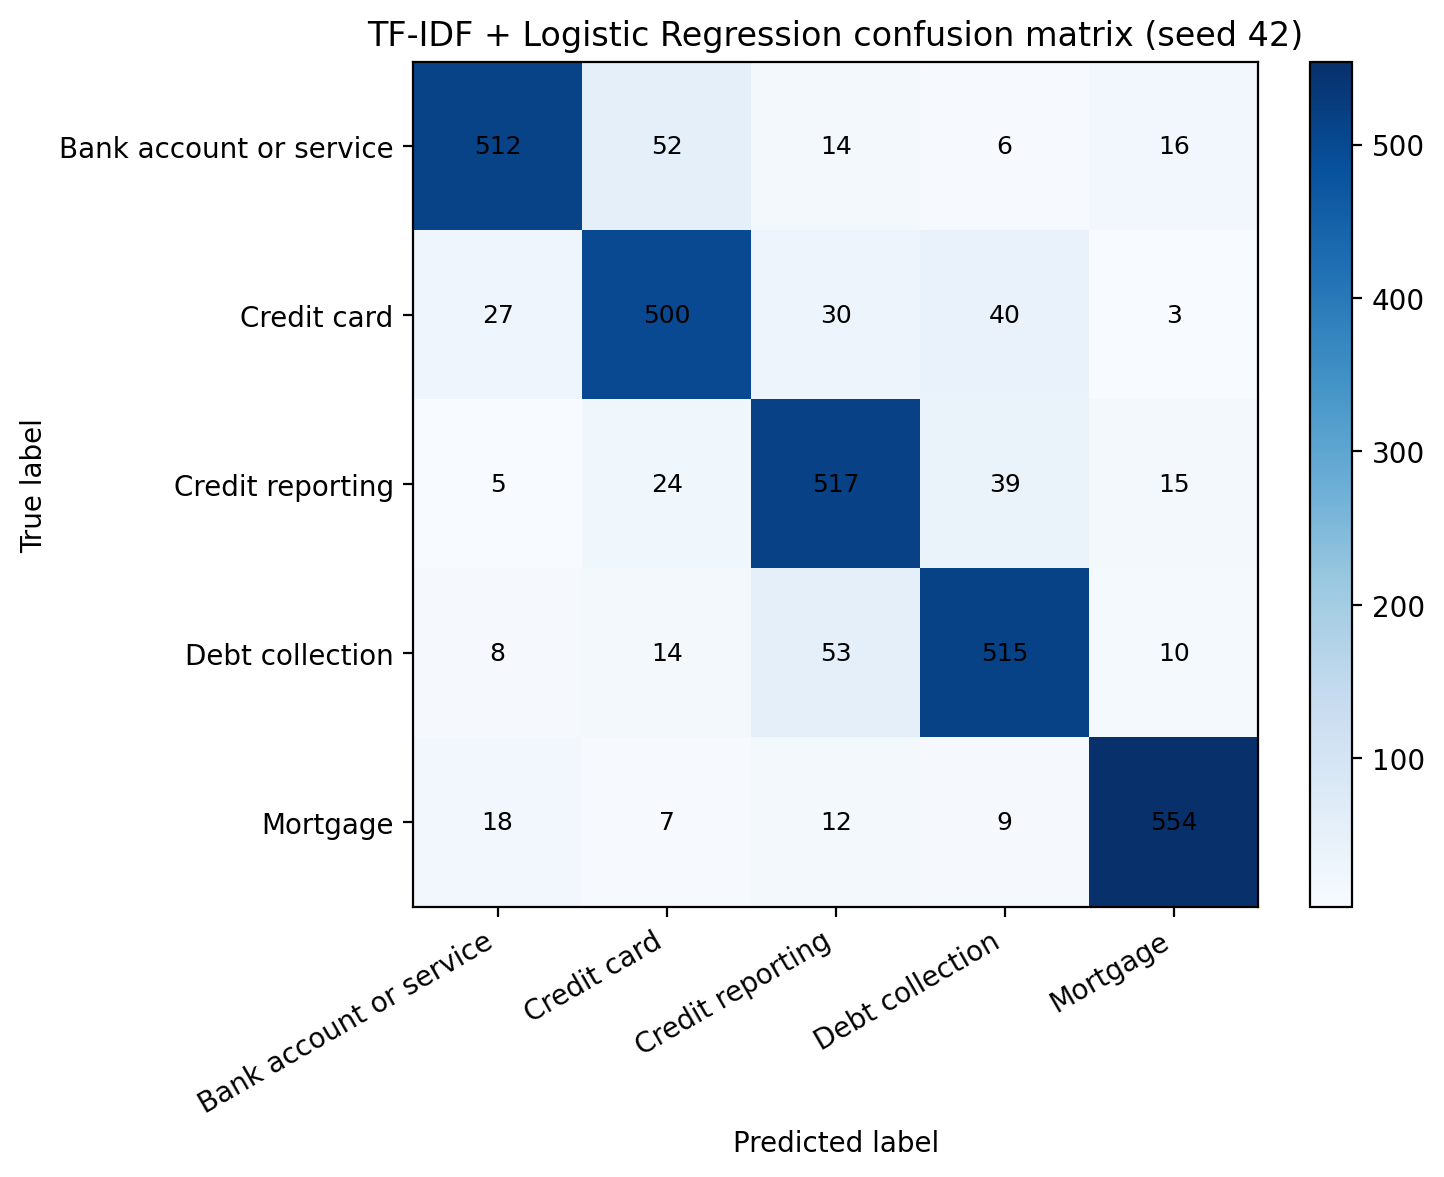
\includegraphics[width=0.76\linewidth]{../artifacts/confusion_matrix_tfidf_seed42.png}

\vspace{0.15cm}
\begin{itemize}
    \item The largest confusion is \textbf{Debt collection $\leftrightarrow$ Credit reporting}.
    \item \textbf{Bank account or service} is also frequently confused with \textbf{Credit card}.
    \item \textbf{Mortgage} is comparatively easiest to identify.
\end{itemize}
\end{frame}

\begin{frame}{Why These Errors Happen}
\begin{itemize}
    \item \textbf{Debt collection vs Credit reporting:} many complaints discuss collection accounts through the lens of credit-report damage, so both label vocabularies appear together.
    \item \textbf{Bank account vs Credit card:} narratives about payments, fees, credit lines, and bank-issued cards blur the boundary.
    \item \textbf{Mortgage vs Bank account:} escrow, autopay, and home-equity complaints sometimes use generic banking language.
\end{itemize}

\vspace{0.25cm}
\textbf{Interpretation:} the strongest remaining mistakes are mostly boundary cases, not random failures.
\end{frame}

\begin{frame}{Conclusion}
\begin{itemize}
    \item TF--IDF + Logistic Regression outperforms both embedding-based models at every dataset size.
    \item Local Word2Vec consistently beats Pretrained GloVe, showing the value of \textbf{domain-specific representations}.
    \item The task is highly \textbf{lexicalized}: sparse features with bigrams are extremely effective.
    \item Repeated runs and the error analysis make the conclusions more credible.
\end{itemize}

\vspace{0.35cm}
\centering
\Large \textbf{Main takeaway:}\\[0.15cm]
Simple classical baselines remain very strong on applied NLP tasks with rich lexical cues.
\end{frame}

\end{document}
